%\documentclass{beamer}
\documentclass[handout]{beamer}

\usepackage[brazilian]{babel}
\usepackage[utf8]{inputenc}
\usepackage{graphicx}
\usepackage{fontenc}
\usepackage{listings}
\usepackage{verbatim}
\usepackage{pxfonts}
\usepackage{graphicx}
\usetheme{Warsaw}

\title{Grandes Migrações}
\subtitle{Passando de Qualquer Plataforma \\
  Para o WordPress}
\author{Vinicius Massuchetto}
\institute{WordCamp Curitiba 2012}
\date{Junho de 2012}

\lstset{%
  breakatwhitespace,
  columns=fullflexible,
  keepspaces,
  breaklines,
  tabsize=2,
  showstringspaces=false,
  extendedchars=true,
  basicstyle=\footnotesize\ttfamily,
  frame=leftline}

\begin{document}

\frame{\titlepage}

\section{Introdução}

\subsection{Introdução}

\begin{frame}{Download}
  \begin{center}
    Esta apresentação está disponível em: \\
    \url{https://github.com/viniciusmassuchetto/wordpress-presentation-migrations}
  \end{center}
\end{frame}

\begin{frame}{Sobre o Que Falaremos}
\begin{itemize}
  \item Por que tratar do assunto
  \item Migrações no WordPress
  \item Migrações em plaraformas suportadas
  \item Migrações de outras plataformas
  \item Estratégias de migração
\end{itemize}
\end{frame}


\subsection{Motivação Para o Cliente}

\begin{frame}{Por que falar sobre migrações com o Cliente?}
\begin{itemize}
  \pause \item Indexação de conteúdo
  \pause \item Manutenção de usabilidade
  \pause \item Reestruturação do conteúdo
\end{itemize}
\end{frame}

\subsection{Motivação Para a Equipe de Desenvolvimento}

\begin{frame}{Por que falar sobre migrações com a equipe de desenvolvimento?}
\begin{itemize}
  \pause \item Análise de complexidade
  \pause \item Análise de correlação e criação de estruturas
  \pause \item Resolução de velhos problemas
  \pause \item Definição de estratégias
  \pause \item Delegação de tarefas
  \pause \item Elaboração de manuais
  \pause \item Definição do tempo de projeto
\end{itemize}
\end{frame}

\subsection{Na verdade..}

\begin{frame}{E na verdade, as migrações são..}
\begin{itemize}
  \pause \item Uma etapa de projeto que poderia ser melhor discutida
  \pause \item Uma das partes mais importantes da implantação de projetos web
\end{itemize}
\end{frame}


\section{Sistemas}

\begin{frame}
\frametitle{O que são migrações para o WordPress?}
\begin{itemize}
  \pause \item WordPress $\rightarrow$ WordPress
  \pause \item Plataformas Suportadas $\rightarrow$ WordPress
  \pause \item Outras Plataformas $\rightarrow$ WordPress
\end{itemize}
\end{frame}

\subsection{WordPress $\rightarrow$ WordPress}

\begin{frame}{WordPress $\rightarrow$ WordPress}
\begin{itemize}
  \pause \item Geralmente tranquila quando feita corretamente
  \pause \item Requere menos processamento e recuperação de conteúdos
               externos
  \pause \item Casos:
    \begin{itemize}
      \pause \item Quando a URL não muda
      \pause \item Quando a URL muda
    \end{itemize}
\end{itemize}
\end{frame}

\begin{frame}{WordPress $\rightarrow$ WordPress: Mesma URL}
\begin{itemize}
  \pause \item Copiar a base
  \pause \item Modificar o \texttt{wp-config.php}
\end{itemize}
\end{frame}

\begin{frame}[fragile]{WordPress $\rightarrow$ WordPress: Mesma URL}
  \lstinputlisting{./code/wp-wp-dump.sh}
\end{frame}

\begin{frame}{WordPress $\rightarrow$ WordPress: URLs Diferentes}
\begin{itemize}
  \pause \item No WordPress, muitas URLs ficam persistentes no banco de dados
  \pause \item Buscar e substituir não resolve
\end{itemize}
\end{frame}

\begin{frame}[fragile]{WordPress $\rightarrow$ WordPress: URLs Diferentes}
  \lstinputlisting{./code/wp-wp-meta.txt}
  \pause
  \lstinputlisting{./code/wp-wp-meta-serialized.txt}
\end{frame}

\begin{frame}[fragile]{WordPress $\rightarrow$ WordPress: URLs Diferentes}
  \lstinputlisting{./code/wp-wp-meta-serialized-replaced.txt}
  \pause
  \lstinputlisting{./code/wp-wp-meta-key.php}
  \pause
  \lstinputlisting{./code/wp-wp-meta-serialized-rep-dump.txt}
\end{frame}

\begin{frame}{WordPress $\rightarrow$ WordPress: URLs Diferentes}
\begin{itemize}
  \item Para mudança de URLs deve-se fazer a substituição
        adequadamente, via plugin ou script
  \pause \item Exemplos:
  \begin{itemize}
    \item Script: Search and Replace Tool
    \item Plugin: WordPress Move
    \item Plugin: Search and Replace
    \item Plugin: WP Migrate Tool
  \end{itemize}
\end{itemize}
\end{frame}

\begin{frame}[fragile]{WordPress $\rightarrow$ WordPress: URLs Diferentes}
  \lstinputlisting{./code/wp-wp-dump.sh}
  e..
\end{frame}

\begin{frame}[fragile]{WordPress $\rightarrow$ WordPress: URLs Diferentes}
  \lstinputlisting{./code/wp-wp-dump-replace-01.sh}
  \pause
  \lstinputlisting{./code/wp-wp-dump-replace-02.sh}
  \pause
  \lstinputlisting{./code/wp-wp-dump-replace-03.sh}
  \pause
  \lstinputlisting{./code/wp-wp-dump-replace-04.sh}
\end{frame}

\begin{frame}[fragile]{WordPress $\rightarrow$ WordPress: URLs Diferentes}
  \lstinputlisting{./code/wp-wp-serialized-replaced.txt}
  \pause
  \lstinputlisting{./code/wp-wp-meta-key.php}
\end{frame}

\begin{frame}[fragile]{WordPress $\rightarrow$ WordPress: URLs Diferentes}
  \lstinputlisting{./code/wp-wp-meta-serialized-replaced-dump.txt}
\end{frame}

\subsection{Sistemas Suportados}

\begin{frame}{WordPress $\rightarrow$ Suportados}
\begin{itemize}
  \pause
  \item Blogger
  \item LiveJournal
  \item Movable Type
  \item RSS
  \item Tumblr
\end{itemize}
\end{frame}

\begin{frame}{WordPress $\rightarrow$ Suportados}
\begin{itemize}
  \item Procedimento direto através de arquivos de exportação
  \pause \item Para mudança de URLs deve-se recorrer a métodos
        similares às migrações WordPress $\rightarrow$ WordPress.
\end{itemize}
\end{frame}


\section{Migrações}

\begin{frame}{Tópicos a Serem Levados em Conta}
  \begin{itemize}
    \pause \item Tecnologia
    \pause \item Estrutura
    \pause \item Referências e relações internas
    \pause \item Conteúdo
    \pause \item Mídias
    \pause \item URLs
  \end{itemize}
\end{frame}

\subsection{Tecnologia}

\begin{frame}{Tecnologias Empregadas}
  \begin{itemize}
    \pause \item Configuração dos servidores\pause \\
                 (safe mode, parâmetros de compilação)
    \begin{itemize}
      \pause \item \texttt{ini\_set("memory\_limit", -1)}
      \pause \item \texttt{set\_time\_limit(0)}
      \pause \item ou.. \pause ajax recursivo
    \end{itemize}
    \pause \item Sistema de banco de dados da estrutura a ser migrada
    \pause \item Modo de obtenção de dados (socket, webservice, csv)
    \pause \item Linguagem a serem escritos os scripts de migração
    \pause \item Preferência: \pause PHP\pause, MySQL\pause, de dentro
                 do WordPress
  \end{itemize}
\end{frame}

\begin{frame}{Tecnologias Empregadas}
  \begin{itemize}
    \pause \item Migrar através do próprio WordPress:
    \begin{itemize}
      \pause \item Facilidade e padronização de manipulação dos dados
      \pause \item Garantia de integridade
    \end{itemize}
  \end{itemize}
\end{frame}

\begin{frame}{Tecnologias Empregadas: wpdb}
  \begin{itemize}
    \pause \item Classe \texttt{wpdb}
    \begin{itemize}
      \pause \item \texttt{query()}
      \pause \item \texttt{get\_results()}
      \pause \item \texttt{get\_var()}
    \end{itemize}
  \end{itemize}
\end{frame}

\begin{frame}{Tecnologias Empregadas: wpdb}
  \lstinputlisting{./code/tec-wpdb.php}
\end{frame}

\begin{frame}{Tecnologias Empregadas: Tratamento}
  \begin{itemize}
    \pause \item Funções de tratamento:
    \begin{itemize}
      \pause \item \texttt{remove\_accents()}
      \pause \item \texttt{sanitize\_title()}
      \pause \item \texttt{normalize\_whitespace()}
      \pause \item \texttt{make\_clickable()}
      \pause \item \texttt{capital\_P\_dangit()}
    \end{itemize}
  \end{itemize}
\end{frame}

\begin{frame}{Tecnologias Empregadas: Abstração de Banco}
    \begin{itemize}
    \pause \item Funções de relação com o banco de dados:
    \begin{itemize}
      \pause \item \texttt{wp\_insert\_post()}
      \pause \item \texttt{wp\_insert\_term()}
      \pause \item \texttt{wp\_set\_post\_terms()}
      \pause \item \texttt{wp\_insert\_attachment()}
      \pause \item \texttt{wp\_update\_attachment\_metadata()}
      \pause \item \texttt{update\_post\_meta()}
    \end{itemize}
  \end{itemize}
\end{frame}

\begin{frame}{Tecnologias Empregadas: Exemplo de Rotina}
  \lstinputlisting{./code/tec-routine.php}
\end{frame}

\begin{frame}{Tecnologias Empregadas: Exemplo de Rotina}
  \lstinputlisting{./code/tec-ajax.php}
\end{frame}

\subsection{Estrutura}

\begin{frame}{Estrutura}
  \begin{center}
    \pause 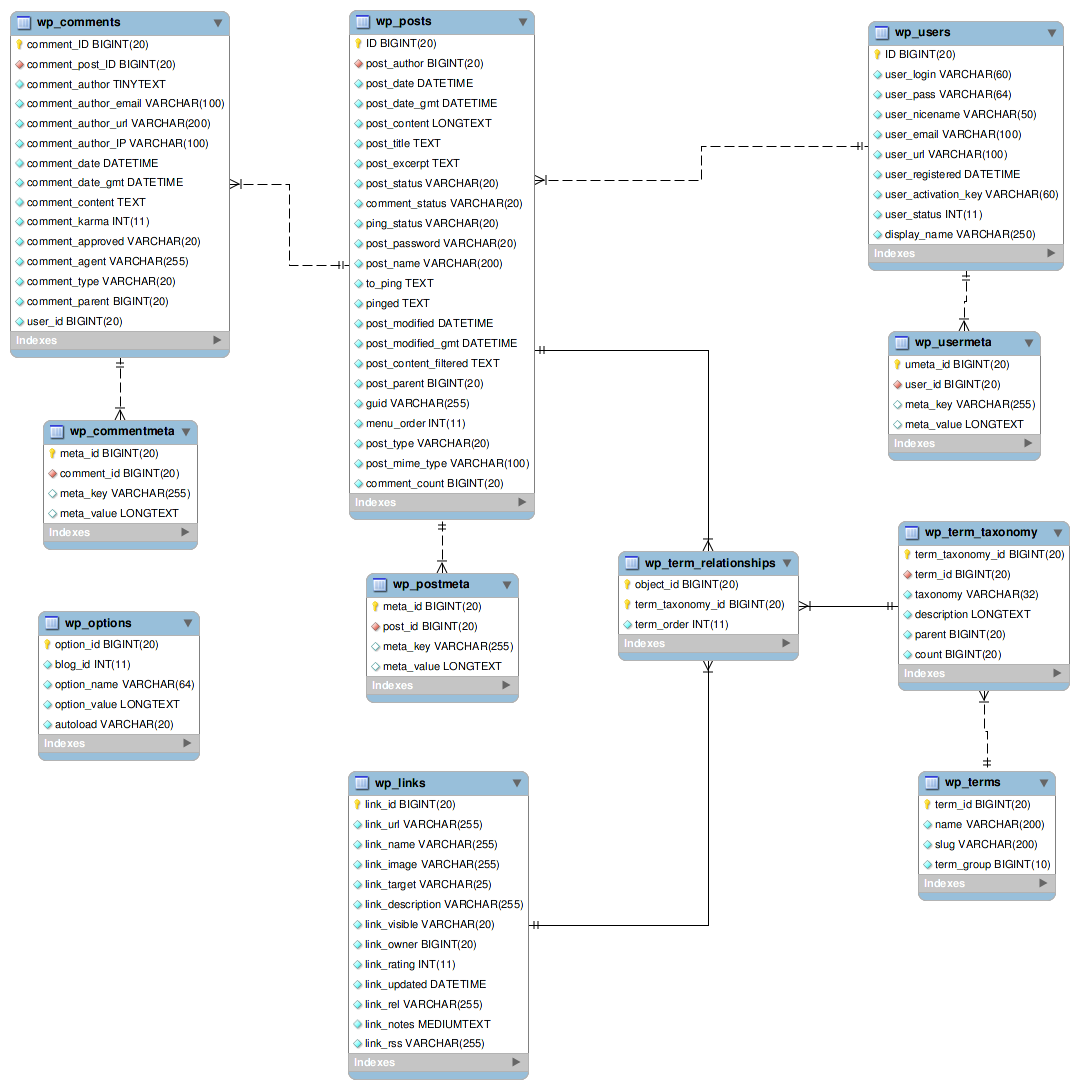
\includegraphics[height=0.8\textheight]{./img/wp-tables.png}
  \end{center}
\end{frame}


\begin{frame}{Estrutura: Mapeamento}
  \begin{itemize}
    \pause \item Identificação das entidades \pause (post types)
    \pause \item Identificação dos atributos \pause (custom fields)
    \pause \item Identificação das relações \pause (taxonomias ou relações de plugins)
  \end{itemize}
\end{frame}

\begin{frame}{Estrutura: Mapeamento}
  Exemplo: Linha de tabela \texttt{estabelecimento}
  \begin{itemize}
    \item \texttt{(int) id}
    \item \texttt{(str) nome}
    \item \texttt{(str) descricao}
    \item \texttt{(str) rua}
    \item \texttt{(str) bairro}
    \item \texttt{(fk)  cidade}
    \item \texttt{(fk)  estado}
    \item \texttt{(fk)  tipo}
    \item \texttt{(fk)  foto}
  \end{itemize}
\end{frame}

\begin{frame}{Estrutura: Mapeamento}
  \begin{itemize}
    \pause \item Post type \texttt{estabelecimento}
    \begin{itemize}
      \item \texttt{post\_title:   nome}
      \item \texttt{post\_content: descricao}
    \end{itemize}
    \pause \item Chaves meta
    \begin{itemize}
      \item \texttt{meta\_key: rua}
      \item \texttt{meta\_key: bairro}
      \item \texttt{meta\_key: \_id}
    \end{itemize}
    \pause \item Taxonomia
    \begin{itemize}
      \item Tipo de Estabelecimento
    \end{itemize}
    \pause \item Anexo
    \begin{itemize}
      \item Foto
    \end{itemize}
  \end{itemize}
\end{frame}

\begin{frame}{Estrutura: Mapeamento}
  \begin{itemize}
    \item \texttt{cidade (??)}
    \item \texttt{estado (??)}
  \end{itemize}
  \pause Soluções possíveis:
  \begin{itemize}
    \item Taxonomia
    \item \texttt{post\_parent}
    \item Relação via custom fields
    \item Relação via plugin \\
          (Advanced Custom Fields, Post Relationships)
  \end{itemize}
\end{frame}

\begin{frame}{Relações Internas}
  \begin{itemize}
    \pause \item Solução depende do escopo de projeto
    \pause \item Algumas transferências devem ser em camadas \\
                 (relações recursivas)
    \pause \item Exemplos:
    \begin{itemize}
      \pause \item Taxonomia ``Tipo de Estabelecimento''
      \pause \item Itens ``Leia também'' de um post
    \end{itemize}
  \end{itemize}
\end{frame}

\begin{frame}{Relações Internas: Inserção sob Demanda}
  \lstinputlisting{./code/ns-get-or-create-category.php}
\end{frame}

\begin{frame}{Relações Internas: Primeira camada de migração}
  \lstinputlisting{./code/ns-migration-layers.php}
\end{frame}


\subsection{Conteúdo}

\begin{frame}{Formatação: Basicamente o conteúdo}
  \begin{itemize}
    \item Elaboração de inventário de conteúdo
    \item Conversão de caminhos
    \item Conversão de embeds em shortcodes
    \item Conversão de estruturas HTML editáveis
    \item Remoção de scripts
  \end{itemize}
\end{frame}

\begin{frame}{Formatação: Capturando Links}
  \lstinputlisting{./code/ns-migrating-links.php}
\end{frame}


\subsection{Mídias}

\begin{frame}{Migração de Mídias}
  \begin{itemize}
    \pause \item Não se contentar com as mídias inseridas no conteúdo
    \begin{itemize}
      \pause \item Sem rastreabilidade pelo software
      \pause \item Sujeitas à estrutura própria de armazenamento
    \end{itemize}
    \pause \item Montar também a biblioteca de mídias e galerias do conteúdo
  \end{itemize}
\end{frame}

\begin{frame}{Migração de Mídias}
  \lstinputlisting{./code/ns-migrating-media-01.php}
\end{frame}

\begin{frame}{Migração de Mídias}
  \lstinputlisting{./code/ns-migrating-media-02.php}
\end{frame}

\begin{frame}{Migração de Mídias}
  \lstinputlisting{./code/ns-migrating-media-03.php}
\end{frame}

\begin{frame}{Migração de Mídias: Serviço Dinâmico}
  \begin{itemize}
    \item Ao invés do download pode-se fazer o serviço dinâmico de mídias.
          Veja o arquivo \\
          \texttt{wp-includes/ms-files.php}
  \end{itemize}
\end{frame}

\begin{frame}{Migração de Mídias: Serviço Dinâmico}
  \lstinputlisting{./code/ns-migrating-media-dynamic-rr.txt}
\end{frame}

\begin{frame}{Migração de Mídias: Serviço Dinâmico}
  \lstinputlisting{./code/ns-migrating-media-dynamic.php}
\end{frame}


\subsection{URLs}

\begin{frame}{URLs}
  \begin{itemize}
    \item Para cada conteúdo migrado, sempre guardar a referência
          para o conteúdo antigo
    \pause \item Na nova estrutura, verificar os meios de acesso no conteúdo
           e redirecionar para o novo.
    \pause \item Casos:
    \begin{itemize}
      \item A partir de referências \texttt{\$\_REQUEST}
      \item A partir de regras de URL
    \end{itemize}
  \end{itemize}
\end{frame}

\begin{frame}{URLs: Referências \texttt{\$\_REQUEST}}
  \lstinputlisting{./code/url-request.php}
\end{frame}

\begin{frame}{URLs: Referências a partir de regras}
  \lstinputlisting{./code/url-rewrite-01.php}
\end{frame}

\begin{frame}{URLs: Referências a partir de regras}
  \lstinputlisting{./code/url-rewrite-02.php}
\end{frame}

\begin{frame}{URLs: Referências a partir de regras}
  \lstinputlisting{./code/url-rewrite-03.php}
\end{frame}


\section{Considerações Finais}

\begin{frame}{Considerações Finais}
  \begin{itemize}
    \item Migrações devem definitivamente ser incluídas como
          componentes de projeto
    \item O WordPress oferece um bom conjunto de ferramentas
          para se trazer dadaos para dentro de sua estrutura.
    \item É cabível o desenvolvimento de plugins específicos
          para a migração de diferentes estruturas
  \end{itemize}
\end{frame}

\begin{frame}{Referências}
\begin{itemize}
  \footnotesize
  \item Codex: Moving WordPress \\
        \url{http://codex.wordpress.org/Moving_WordPress}
  \item GitHub / interconnectit / Search-Replace-DB \\
        \url{https://github.com/interconnectit/Search-Replace-DB}
\end{itemize}
\end{frame}

\end{document}
